\section{\ac{TMI} Minicore}
\label{sec:tmi_minicore}

\subsection{Problem Statement}
\label{subsec:tmi_minicore_ps}

The previous two problems dealt with relatively simple functions that don't require industrial engineering codes to solve. However, the main intention of this thesis is to construct reduced order models for computer codes that aim to model large and complex engineering systems. Interaction with such computer codes consist of input and output files; the governing equations and their solvers are rarely seen. The primary purpose of this demonstration problem is to show that the same algorithms applied to analyze the previous problems are also functional when applied to engineering computer codes.

In this demonstration problem the reactor core simulator code \ac{PARCS} \cite{PARCS} is applied to the \ac{TMI} minicore described in the first phase of the \ac{UAM} Benchmark \cite{UAM_Benchmark}. The minicore problem consists of a three-by-three fuel assembly configuration with reflector blocks placed around the assemblies, as seen in Figure \ref{fig:tmi_minicore}. In the minicore the central assembly is rodded while the periphery fuel assemblies are unrodded. Vacuum boundary conditions are applied. The few-group, homogenized cross section description for each fuel assembly consists of transport, absorption, nu-fission, and scatter cross sections along with values for \ac{ADFs}. For a two-group problem the total number of cross sections to describe an assembly is nine. Since the homogenized reflector region does not support fission only seven homogenized cross sections are required to describe it. Consequently, to model the minicore configuration in Fig. \ref{fig:tmi_minicore} in \ac{PARCS} a total of twenty five homogenzied, two-group cross sections are needed.  
\begin{figure}[!htb]
\caption{\label{fig:tmi_minicore}
\ac{TMI} minicore configuration used for analysis, as defined in the \ac{UAM} Benchmark specifications.}
 \begin{center}
  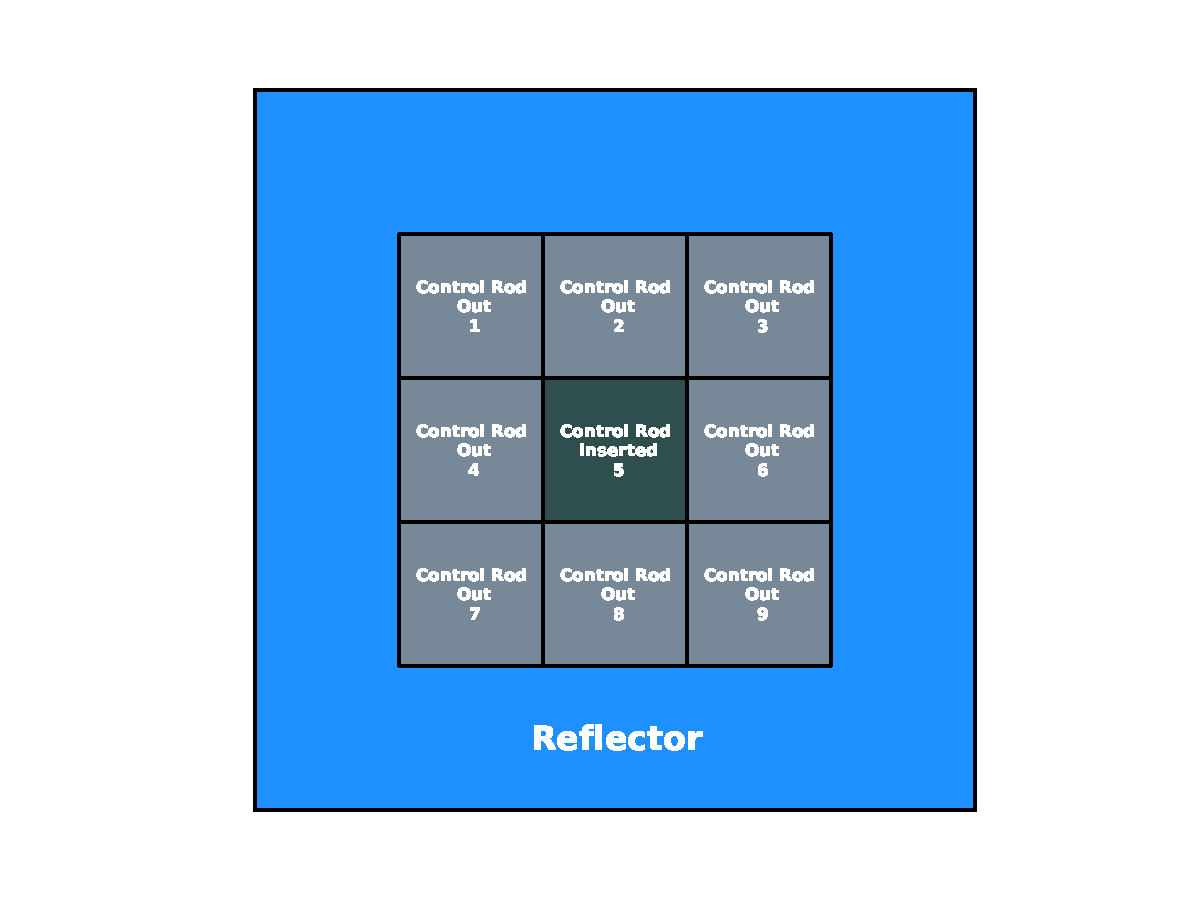
\includegraphics[scale=.75]{./Chapter3/tmi_minicore.pdf}
 \end{center}
\end{figure}  

In order to study the effects of the uncertainties inherent in the few-group cross sections on output parameters of interest in \ac{PARCS}, a few-group covariance matrix is necessary. The few-group covariance matrix is obtained using the 'two-step' method depicted in Fig. \ref{fig:sampler_flow_diagram}. A total of 300 transport calculations with perturbed multigroup cross sections were executed to generate the few-group covariance matrix. In the previous example problems only one output parameter was investigated at a time. However, recall in the discussion of the Smolyak algorithm that interpolation is only performed on the random space. The objective function is evaluated at each abscissa in the random space, returning an output that can still be a function of physical space. In this case the hierarchical surplus is no longer one dimensional. Rather, the hierarchical surplus in Eq. \ref{eq:hierarchical_surplus} is rewritten as,
\begin{equation} 
\label{eq:hierarchical_surplus_space}
   f(\mathbf{x}, x_{j_1}^{i_1},...,x_{j_d}^{i_d}) - 
    A(q-1,d)(\mathbf{x}, x_{j_1}^{i_1},...,x_{j_d}^{i_d})
\end{equation}
where $\mathbf{x} \in \mathcal{D}$ is a coordinate in the spatial domain. When the objective function is a function of spatial coordinates the Smolyak algorithm approximates the function as a linear combination of vectors, the linear weights still being tensor products of basis functions for the random space. To determine the mean and variance of a reduced order model approximation of some space-dependent objective function the $L_2$ norm is taken over the spatial domain $\mathcal{D}$. Similarly, to identify important dimensions using the sensitivity coefficient defined in Eq. \ref{eq:anova_sensitivity} the $L_2$ norm is taken of $\eta_i(\mathbf{x})$.  

The problem in this section considers the core box power distribution of the minicore in Fig. \ref{fig:tmi_minicore} and consequently, the objective function is space dependent. For each simulation in \ac{PARCS} a vector of length nine is returned with each entry containing the relative box power in the fuel assemblies. The box powers are calculated such that the average of all nine entries is identically equal to unity. In the \ac{PARCS} output file the box powers are only given to four digits of accuracy and therefore roundoff error in this problem warrants some attention.  

\subsection{Analysis}
\label{subsec:tmi_analysis}

In this analysis a pure 'two-step' approach is used to compare the results obtained using a reduced order model for the box powers output in \ac{PARCS}. For the 'two-step' approach a few group covariance matrix is constructed and sampled 500 times, with each sample containing perturbed few group cross sections. Each cross section set is propagated through the \ac{PARCS} code and the box powers for the fuel assemblies are extracted from the output file. Ultimately, 500 box power outputs are analyzed statistically to obtain correlations, means, and variances. The same few group covariance matrix is used to sample the reduced order model for the box powers.    

To build a reduced order model, Algorithm \ref{code:rom_algorithm} is applied with a hierarchical surplus threshold of $10^{-4}$ since the \ac{PARCS} box powers are only output to four decimal places. Consequently, roundoff error may accumulate in the fourth decimal point of the reduced order model. A total of 123 executions of \ac{PARCS} were required to construct all single order components of the reduced order model using Clenshaw-Curtis abscissas. Due to the geometry of the \ac{TMI} minicore, 1/8 symmetry is expected in the box power results. Consequently, only fuel assemblies one, four and five are investigated, as defined in Fig. \ref{fig:tmi_minicore}. Sampling results for the mean and standard deviation for the true box power \ac{PARCS} model and the reduced order model are summarized in Tables \ref{table:tmi_mean_sd_mc} and \ref{table:tmi_mean_sd_1d}, respectively. 
%
\begin{table}[!htb] 
\caption{\label{table:tmi_mean_sd_mc} 
Mean and standard deviation data for \ac{TMI} minicore box powers where \ac{PARCS} code is used as objective function. A total of 500 samples were used. Assembly numbers correspond to Fig. \ref{fig:tmi_minicore}.}
\centering
\begin{tabular}{||c|c|c|c|c||} 
\hline \hline
\textbf{Assembly} & \textbf{Mean} & \textbf{99\% CI} & \textbf{Standard Dev.} & \textbf{99\% CI} \\ \hline
1 & 0.8387 & (0.8386, 0.8388) & 0.0007 & (0.0006, 0.0008) \\ \hline 
2 & 1.1499 & (1.1498, 1.1500) & 0.0011 & (0.0010, 0.0012) \\ \hline
3 & 0.8387 & (0.8386, 0.8388) & 0.0007 & (0.0006, 0.0008) \\ \hline
4 & 1.1499 & (1.1498, 1.1500) & 0.0011 & (0.0010, 0.0012) \\ \hline
5 & 1.0453 & (1.0450, 1.0456) & 0.0027 & (0.0025, 0.0029) \\ \hline
6 & 1.1499 & (1.1498, 1.1500) & 0.0011 & (0.0010, 0.0012) \\ \hline
7 & 0.8387 & (0.8386, 0.8388) & 0.0007 & (0.0006, 0.0008) \\ \hline
8 & 1.1499 & (1.1498, 1.1500) & 0.0011 & (0.0010, 0.0012) \\ \hline
9 & 0.8387 & (0.8386, 0.8388) & 0.0007 & (0.0006, 0.0008) \\ 
\hline \hline
\end{tabular}
\end{table}
%
\begin{table}[!htb] 
\caption{\label{table:tmi_mean_sd_1d} 
Mean and standard deviation data for \ac{TMI} minicore box powers where the objective function is a reduced order model for \ac{PARCS} containing only 1D components. A total of 500 samples were used. Assembly numbers correspond to Fig. \ref{fig:tmi_minicore}.}
\centering
\begin{tabular}{||c|c|c|c|c||} 
\hline \hline
\textbf{Assembly} & \textbf{Mean} & \textbf{99\% CI} & \textbf{Standard Dev.} & \textbf{99\% CI} \\ \hline
1 & 0.8387 & (0.8386, 0.8388) & 0.0007 & (0.0006, 0.0008) \\ \hline 
2 & 1.1500 & (1.1499, 1.1501) & 0.0012 & (0.0011, 0.0013) \\ \hline
3 & 0.8387 & (0.8386, 0.8388) & 0.0007 & (0.0006, 0.0008) \\ \hline
4 & 1.1500 & (1.1499, 1.1501) & 0.0012 & (0.0011, 0.0013) \\ \hline
5 & 1.0455 & (1.0452, 1.0458) & 0.0027 & (0.0025, 0.0029) \\ \hline
6 & 1.1500 & (1.1499, 1.1501) & 0.0011 & (0.0010, 0.0012) \\ \hline
7 & 0.8387 & (0.8386, 0.8388) & 0.0007 & (0.0006, 0.0008) \\ \hline
8 & 1.1500 & (1.1499, 1.1501) & 0.0012 & (0.0011, 0.0013) \\ \hline
9 & 0.8387 & (0.8386, 0.8388) & 0.0007 & (0.0006, 0.0008) \\
\hline \hline
\end{tabular}
\end{table}
%
As always, the same random numbers are used to produce each sample when comparing two different methods. The results are identical in all cases to four significant digits and in most cases, to five significant digits. In the reduced order model results notice that the standard deviation for assembly six is slightly off in the fourth decimal place when compared to assemblies two, four, and eight. The standard deviation should be equal in these four assemblies due to symmetry, indicating the presence of roundoff error.        

Adding higher order components in accordance with Algorithm \ref{code:rom_algorithm} did not improve the statistics of the reduced order model. For the purposes of uncertainty quantification the reduced order model consisting entirely of 1D components is sufficient for this problem. The bivariate distributions for the box powers for all combinations of assemblies one, four, and five are given in Fig. \ref{fig:tmi_correlations}.    
\begin{figure}[!htb]
\caption{\label{fig:tmi_correlations}
Multivariate distributions for the box powers of two assemblies. Dashed distributions were obtained by sampling the reduced order model consisting of only 1D components.}
 \begin{center}
  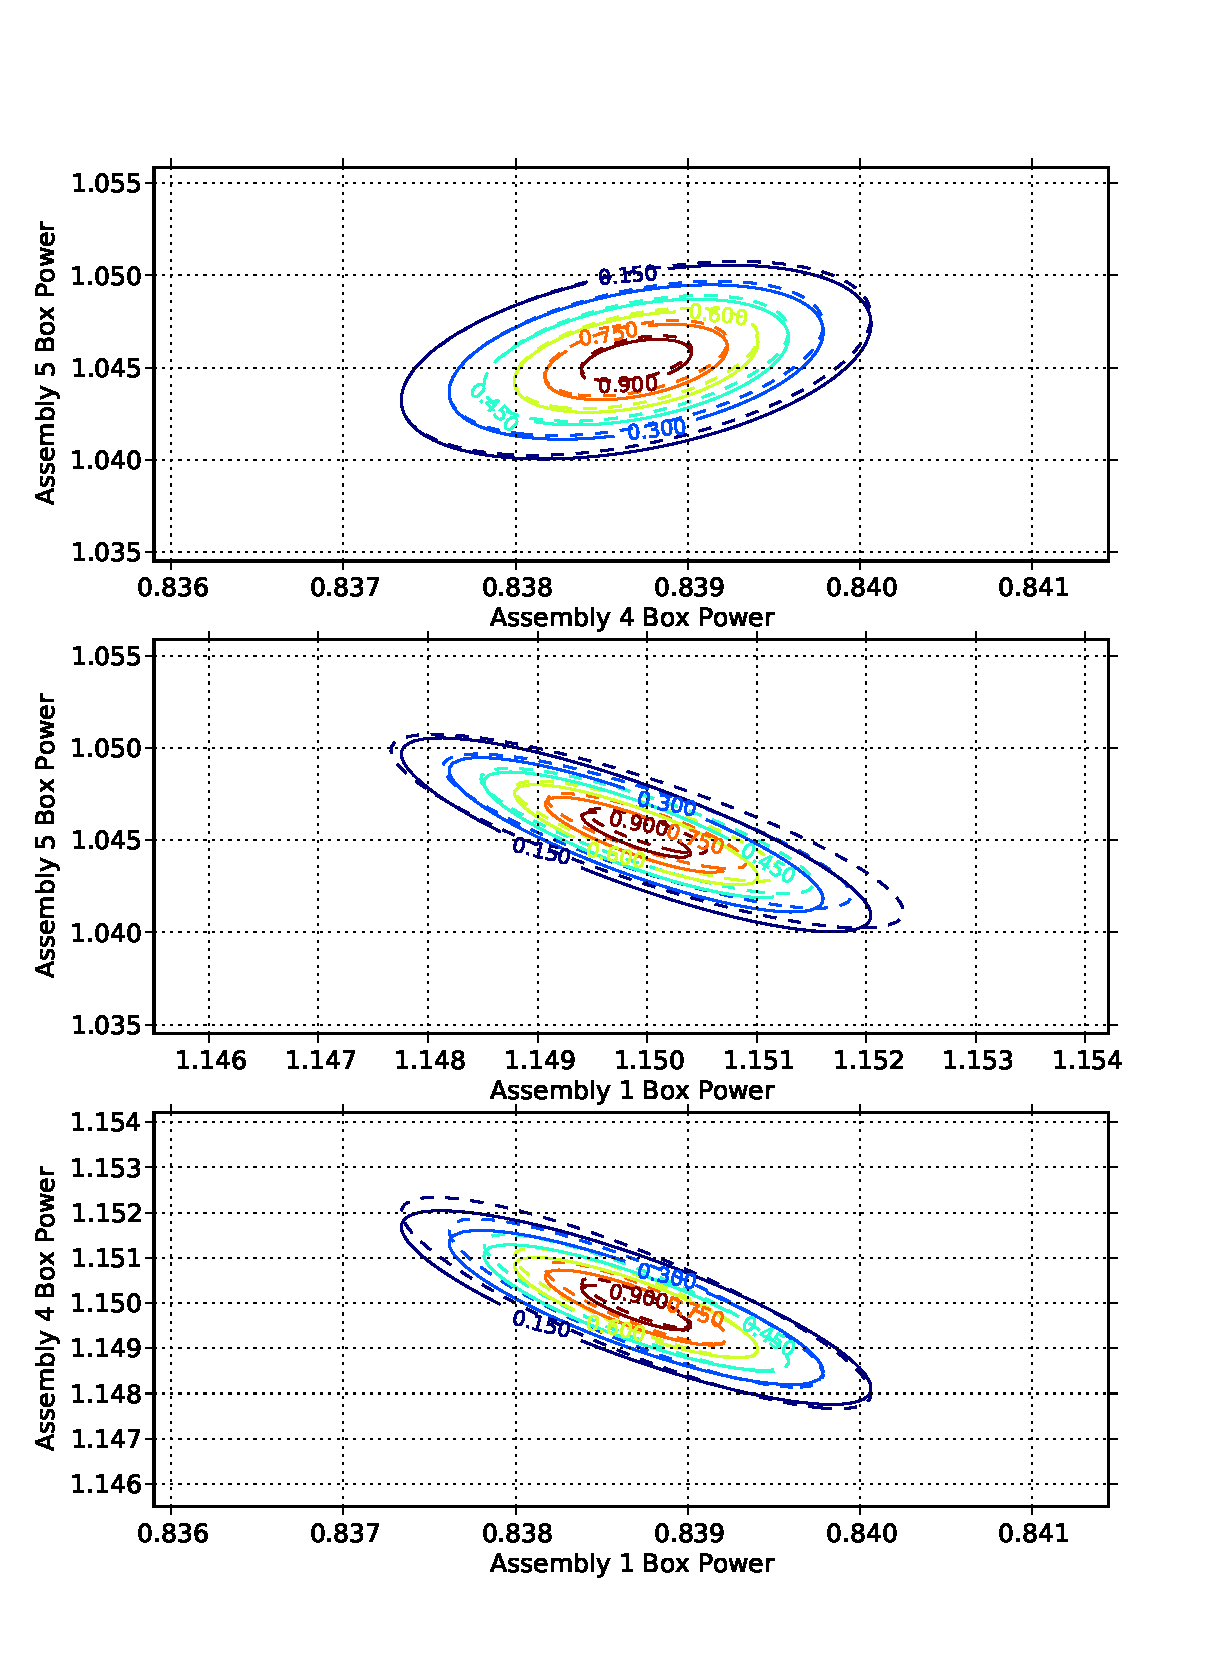
\includegraphics[scale=.70]{./Chapter3/tmi_correlations.pdf}
 \end{center}
\end{figure} 
For each case in Fig. \ref{fig:tmi_correlations} the bivariate distributions are obtained by sampling the reduced order model and \ac{PARCS}. Variations between the overlayed distributions can be attributed to roundoff error. A decrease in the box power of assembly five is equivalent to an increase in the absorption of the assembly's control rods, which effectively shifts the neutron flux away from the central assembly. Consequently, a negative correlation is expected between assemblies one and five and between assemblies one and four. Indeed, statistical sampling has the Pearson correlation coefficient for the box powers of assemblies one and four to be $-0.83$ and $-0.84$ between assemblies one and five. However, negative correlation coefficients between assembly one and assemblies four and five implies a positive correlation coefficient between assemblies four and five. The positive correlation coefficient of $+0.40$ between assemblies four and five is evident in Fig. \ref{fig:tmi_correlations}.  

